\subsection{Sequence Diagram}
I \textbf{diagrammi di sequenza} (o Sequence Diagram) descrivono attraverso notazione grafica come gli oggetti interagiscono tra di loro per realizzare un certo comportamento. Sono composti da:
\begin{figure}[h]
    \centering
    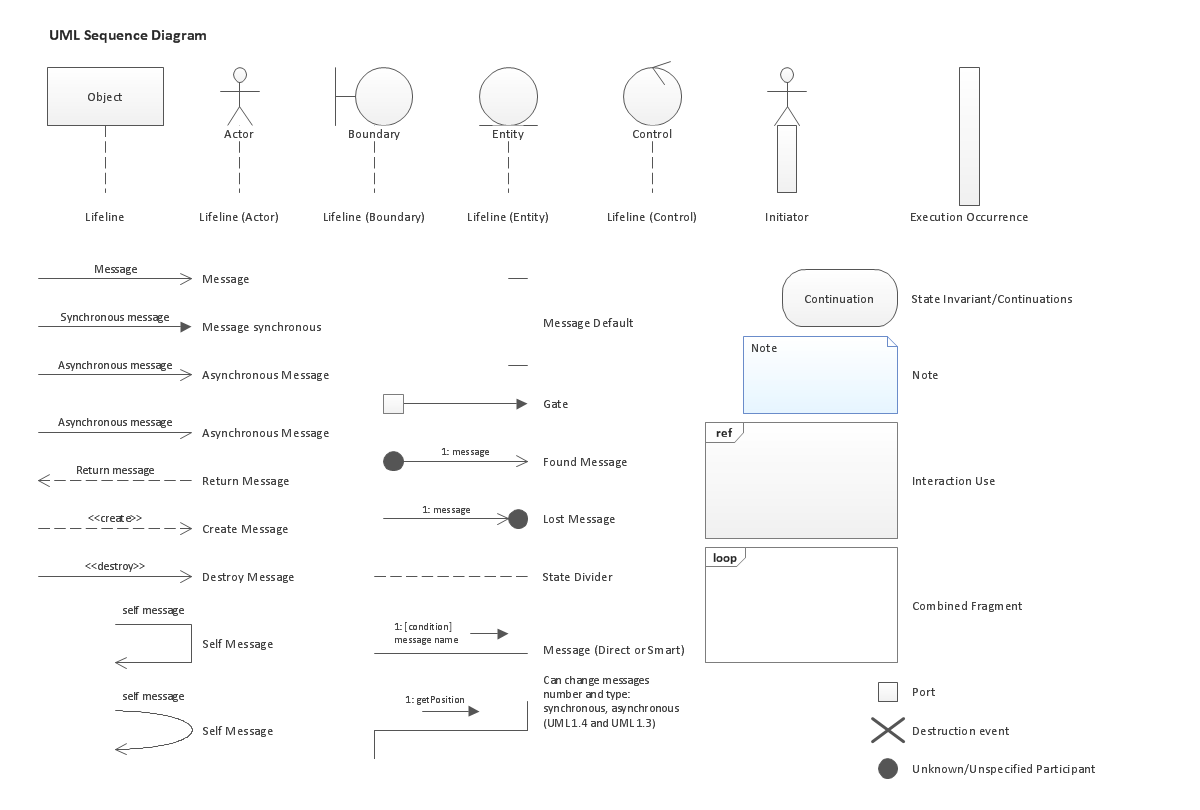
\includegraphics[width=1\linewidth]{IDSTEORIA/Immagini/UML/UMLSequenceDiagramElements.png}
    \caption{Notazione grafica dei vari elementi del Sequence Diagram.}
    \label{fig:seq_elements}
\end{figure}
\begin{itemize}
    \item \textbf{Linee di vita (o lifelines)}, oggetti o classi coinvolte nell'interazione, sono rappresentati da un rettangolo contenente le informazioni base (nome, tipo) e da una linea verticale rappresentante la durata dell'esistenza nel sistema.
    \item \textbf{Messaggi}, sono l'interazione tra due lifeline. Possono essere:
    \begin{itemize}
        \item Chiamate di operazione 
        \item Risposte
        \item Chiamate di creazione/distruzione
    \end{itemize}
\end{itemize}


Ulteriori approfondimenti sulle norme per realizzare i Sequence Diagram nell'\hyperref[appendix:sequence]{apposita appendice}.